\documentclass[journal]{IEEEtran}
% \usepackage{times}
% \usepackage[small,compact]{titlesec}
% \usepackage[small,it]{caption}
% \usepackage{natbib}
% \usepackage{fullpage}
\usepackage{graphicx}
\usepackage[cmex10]{amsmath}
\interdisplaylinepenalty=2500

\title{EECS 592 Final Progject: 3D Depth Reconstruction with Monocular Vision using Supervised Learning}
\author{Yiying Li}
\date{\today}

\begin{document}
\maketitle

\begin{abstract}
Generating depth from monocular vision (single image) is an interesting problem that humans solve fairly well. I replicated the work of Saxena et al. \cite{saxena2008} which takes a supervised learning approach. A training set is provided online containing various environments, such as indoor rooms, forests, building, etc, matched with their corresponding ground truth depth map generated by a 3D laser scanner system. Current research shows that depth estimation using a single image is difficult since local features of the image are insufficient, and global context is hard to define statistically. The algorithm implemented uses a hierarchical, Markov Random Field to model the image features to incorporate both local features as well as global context. Stereo vision can be augmented by this method to improve the areas in which stereo vision has difficulties, since monocular features and stereo geometric features are largely orthogonal. The current result of the reproduction is in progress, and the abstract will be updated to provide a short comparison in the final report.
\end{abstract}

\section{Introduction}
There is a lot of research on 3D reconstruction, and depth estimation using monocular vision. Most of them uses stereopsis vision \cite{scharstein2003}, or multiple images. Some also require multiple images, such as structure from motion \cite{Forsyth:2002:CVM:580035}. All of these focus on geometric differences that incorporate the use of triangulation. Humans can detect a lot of depth with one eye using monocular cues such as gradients, focus, coloring, and others. We also use these monocular cues along with stereo ones to figure out depth for ourselves. 

Depth estimation is still extremely difficult on a single still image, since there are a lot of ambiguity in local features. The algorithm must try and exploit some characteristic of the global structure of the image as well as try to use past experiences to augment the data. Depth extraction is extremely important to an overall bigger picture of scene understanding. 

\section{Visual Cues}
The visual cues that humans use are grouped into four categories by previous research \cite{loomis01, schwartz99}, monocular, stereo, motion parallax, and focus cues. We combine these to understand the 3D structure of the world, the model will try to combine most of the monocular cues and stereo cues to estimate depth.

Monocular cues are important to the estimation of depth. Texture gradients help capture the distribution of edge directions, which in turn indicate depth on a certain scale. A classic example is a tiled floor with parallel lines could appear to have tilted lines in an image. Haze is caused by light scattering which is another cue that certain objects are further away. There are many other cues such as occlusion, defocus, shading, shadows, etc. Most monocular cues are information of the global properties of the image, and thus can't be computed or inferred from local regions in the image, even if certain local information such as color could be an indicator. Overall properties of the entire image must be looked at to try and capture these monocular cues.

As a robot moves, close objects appear to move more than objects that are further away. This is an example of motion parallax cues. The ability to focus also causes certain object to be out of focus, this can be an indicator of depth as well. Stereo cues usually rely on some sort of geometric relation between the two cameras capturing the images. There is a downfall to stereo cues for object at distances extremely far away, it is hard to generate the relationship when you get to sub-pixel differences.

\section{Feature Extraction}
The image is divided into small rectangular patches, and a single depth value is estimated for each patch. There are two types of features used in this estimate, {\em absolute} depth features are used to estimate the depth at the specific depth and {\em relative} features which are used to estimate relative depth. Relative depth is the magnitude of the difference between the two patches. Absolute features map to local feature processing and relative features maps to continuity features for humans.

\begin{figure*}[!t]

\includegraphics[width=\linewidth]{lawsmask.PNG}
\caption{The first 9 are laws' mask, and the rest are rotated edge detectors}
\label{fig:lawsmask}
\end{figure*}

\begin{figure*}[!t]
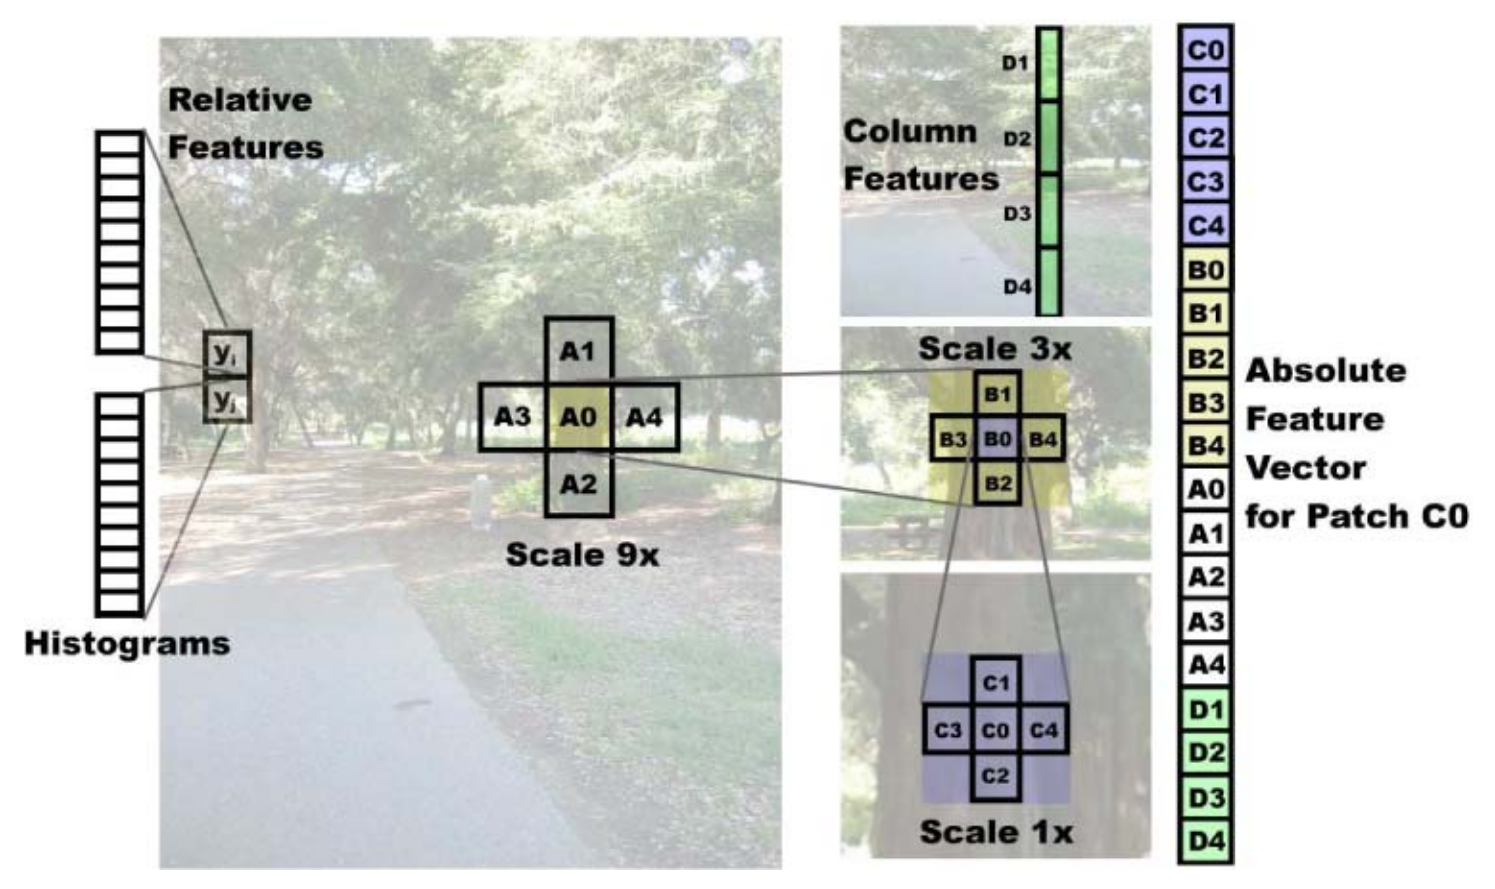
\includegraphics[width=\linewidth]{Features.PNG}
\caption{The absolute depth features vector is generated from the textual energies of a patch, its surrounding patches, the textual energies of the different scale patches centered on this patch, their surrounding patches, and the textual energies of vertical column patches. The relative features for each patch is a histogram of the different textual energies.}
\label{fig:featureimage}
\end{figure*}

Three types of local cues are captured: texture variation, texture gradients, and color. Texture variation is mostly contain in the intensity of the image, therefore we store the image in the YCbCr color format so we can isolate this channel. Laws' mask \cite{davies04, michels05} can be applied to this channel to compute texture energy (Figure \ref{fig:lawsmask}). Haze can be calculated by first applying the first Laws' mask, which is a local averaging filter, to each of the color channels. Texture gradients that are resistant to noise can be generated with size oriented edge filters. We split these features into absolute depth features and relative depth features. We calculate these textural energy on a patch of a certain size, we also have different scales for the patch size which can be see in Figure \ref{fig:featureimage}.

\subsection{Absolute Depth Features}
(need to add a image explaining how this works)

For each patch $i$ inside an image $I(x, y)$, where $x, y$ correspond to location of the patch. There are 17 outputs from the the filters (9 Laws' masks, 2 color, 6 texture gradients). Let these filter outputs be represented by $F_n, n = 1,..., 17$. Then the energy of each filter is calculated by
\begin{equation}
E_i(n, k) = \sum_{(x, y) \in patch(i)} |I * F_n|^k
\end{equation}
where $k \in \{1, 2\}$, this generates a feature vector of 34 elements.
This isn't enough as we need to incorporate more of the global properties. The author mentions that using more $k$ values doesn't affect the results at all. This is done by extract on multiple image resolutions. To capture these properties the features are computed from the neighboring four patches as well as the current patch. This is then repeated on 3 different scales (resolutions) and the neighbors on each scale. We also add a column vector that contains 4 column patches to account for vertical consistency. The column vector is size at the highest scale in order to capture the most potential consistency of the object. The full feature vector for this patch comes out to $19*34 = 646$ elements in the each feature vector for each patch.

\subsection{Relative Features}
A 10-bin histogram is calculated for each of the 17 $F_n$ filters, generating $170$ features for each patch at each scale. This is used to estimate the difference in depth between two different locations. This require less global information as if nearly by patches exhibit extremely similar properties then it is somewhat safe to consider them the same object. Relative depth features $y_{ijs}$ for two neighboring patches $i$ and $j$ on scale $s$ can be calculated from the difference of the histograms.

\section{Markov Random Field}
A Markov random field (MRF) is a set of random variables in a undirected graph where the variables have a Markov property. This provides a consistent and convenient way to model things that are context-dependent such as depth features. Nodes in $S$ are related to each other by a neighborhood system $N = \{N_i, i \in S\}$. This can be multi-dimensional and can also be characterized by a Gibbs distribution. There are many ways to train a MRF, the most popular way is to use maximum likelihood either over joint distribution or marginal likelihood.
The maximum joint likelihood can be used to train the Gaussian MRFs, however Laplacian MRFs are intractable using maximum joint likelihood as there is no close form to the partition function. Laplacian MRF's can be roughly estimated using the Gaussian approximation.

MRFs have a variety of uses in computer vision as many tasks can be posed as energy minimization problems on a rectangular grid of pixels. Some examples where MRFs have been used extensively is in problems such as denoising, finding the stereo disparity, reconstruct smooth surface given sparse measurements, and segmentation (aka foreground extraction). The key to using MRFs is that since there are a lot of local connections information from one point can propagate very far into another point on the graph. This is important to try and interpret local information on a global scale. We want to use this key feature for MRFs to try and propagate the local information of patches since even areas far away from each other may have can effect on the depth of those areas.
\section{Models}

\subsection{Gaussian Model}
The Gaussian Markov Random Field model is shown in Equation \ref{eq:gaussian_model}.
\setlength{\arraycolsep}{0.0em}
\begin{eqnarray}
\label{eq:gaussian_model}
P_G(d|X; \theta, \sigma) &{}={}& \frac{1}{Z_G}\exp\left(-\sum_{i=1}^{M}\frac{(d_i(1)-x_i^T\theta_r)^2}{2\sigma^2_{1r}} \vphantom{\sum_{j \in N_s(i)}}\right.\nonumber\\
&&- \left.\sum_{s=1}^3\sum_{i=1}^M\sum_{j \in N_s(i)} \frac{(d_i(s)-d_j(s))^2}{2\sigma_{2rs}^2}\right)
\end{eqnarray}
\setlength{\arraycolsep}{0.0em}

$M$ is the number of patches in the image at the lowest scale, $Z_G$ is the normalization constant, $x_i$ is the absolute depth feature vector for patch $i$, $\theta$ and $\sigma$ are the parameters of the model. These parameters are further parameterized by row $r$, since the images are assume to be taken from a horizontally mounted camera thus exhibiting similar properties. The depths are $d_i(s), s \in \{1, 2, 3\}$, the depth at higher scales are the average of the depths of the lower scales as indicated in Equation \ref{eq:higher_depth}
\begin{equation}
\label{eq:higher_depth}
d_i(s+1) = (1/5)\sum_{j \in N_s(i) \cup {i}} d_j(s)
\end{equation}
$N_s(i)$ are the neighbors of patch $i$ on scale $s$. The second summation term is a smoothing factor that depends on the variance parameters $\sigma_{2rs}^2$ to determine the amount of smoothing.

The variance term $\sigma_{2rs}^2$ is a linear function of patch $i$ and $j$'s relative depth features $y_{ijs}$. This is modeled as $\sigma_{2rs}^2 = u^T_{rs}|y_{ijs}|$, this helps with which neighboring patches are likely to have similar depth. The other variance term $\sigma^2_{1r} = v_x^T x_i$ is a linear function of the features, this gives a uncertainty measure as well as a dependency on features. The variables $u^T_{rs}$ and $v_x^T$ are fitted to their corresponding trained variances. Inference on this network is done with a MAP estimate (need to include the math for this). Log $P(d|X; \theta, \sigma)$ is quadratic, therefore the maximum is easily found.

\subsection{Laplacian Model}
The Laplacian model is show in Equation \ref{eq:laplace-model}.

\setlength{\arraycolsep}{0.0em}
\begin{eqnarray}
\label{eq:laplace-model}
P_L(d|X; \theta, \lambda) &{}={}& \frac{1}{Z_L}\exp\left(-\sum_{i=1}^{M}\frac{|d_i(1)-x_i^T\theta_r|}{\lambda_{1r}} \vphantom{\sum_{j \in N_s(i)}}\right.\nonumber\\
&&- \left.\sum_{s=1}^3\sum_{i=1}^M\sum_{j \in N_s(i)} \frac{|d_i(s)-d_j(s)|}{\lambda_{2rs}}\right)
\end{eqnarray}
\setlength{\arraycolsep}{0.0em}

The reason for this model is that the relative features in the form of a histogram are more Laplacian than Gaussian. This model also has much longer tails than Gaussian, therefore lending itself to be more robust to outliers which also producing sharp edges that the Gaussian model failed to do.

Maximum likelihood is intractable for a Laplacian model, since the partition depends on $\theta_r$. We can approximate by solving linear system of equations $X_r\theta_r \approx d_r$ to minimize $L_1$ norm errors ($min_{\theta_r}(||d_r-X_r\theta_r||_1$). The spread parameters are learned the same way as the Gaussian model except losing the exponents and adding absolute values. MAP inference is still tractable and convex, this can be solved using a linear program.

\section{Replication}
The replication was mostly done in MATLAB for its extensive image processing library, as well as its very optimized set of functions for linear regression as well as robust linear regression where we throw out outliars. As expected there were many difficulties in replication of this work. I will point them out before we get to the results because it is important to understand what couldn't be accomplished before looking at the results. I will break down the difficulties that I was able to overcome and the difficulties that I was not able to overcome. Many of these problems stemmed from insufficient information on the models as well as current hardware limitations. There are a few numbers that they don't provide and assumptions had to be made, the most important is the patch size of the lowest scale. I chose this to be a 8x8 patch as that reduced the 1704x2272 image to 213x284, which was as close as possible to the size of the depth map provided.

\subsection{Surmounted Difficulties}
The first task of feature generation was initially hard as they don't provide the values of the mask's they used for convolution to generate the features of the image. Fortunately Law's mask are a specific set of filters that are readily available in computer vision text book. The rotated edge filters, while the general form of an edge filter is simple, there is a problem of the scale and there is quite a bit of difference between the filter if Eq \ref{eq:filter1} and filter in Eq \ref{eq:filter2}. The scale also can vary the output slightly and potentially causing the regression to lean towards a certain value. I ended up just choosing the filter in Eq \ref{eq:filter1}, as it is more widely used in vision applications. Another problem that occurred with the edge filters is the rotation of the filters, if we just try to rotate these matrices by $30^{\circ}$ then there has to be some interpolation. Filters generally are integral numbers, therefore if use interpolation we have to fix the floating point numbers to integral numbers. When I did this it doesn't line up with what the author has presented in masks (Figure \ref{fig:lawsmask}). What I did was to go back and change all the values of the filters until they matched the output from the author, and I can only assume that I did this correctly as there is no way to know that the author and I chose the same form of visualization (however there isn't many different ways).
\begin{eqnarray}
\label{eq:filter1}
\begin{bmatrix}
	-2~&0~&-2 \\
	-2~&0~&-2 \\
	-2~&0~&-2 \\
\end{bmatrix}
\end{eqnarray}
\begin{eqnarray}
\label{eq:filter2}
\begin{bmatrix}
	-2~&1~&-2 \\
	-2~&1~&-2 \\
	-2~&1~&-2 \\
\end{bmatrix}
\end{eqnarray}

Once I started to do feature extraction I ran into many problems with the speed of the algorithm. Since we have to sum over all the pixels an extreme number of times as we have many patches and for each patch we also had to account for surrounding patches. With a very naive implementation this would have taken around 400 hours (16 days) for 400 images. I had to think of much more efficient way to calculate this, as the author doesn't tell you how to do this as I think this pretty far into implementation details. I still feel it is important to state how important and how much time it could have saved me if the author mentioned pre-computing certain things. With pre-computing the patches at only the lowest scale and a clever pre-computing on for the columns, I was able to achieve 100 seconds per image.

Running regression on the model for learning posed another interesting yet annoying and non-technical problem. The resulting features data from a single 1704x2272 images was around 280MB of data. If we wanted to train on 400 images, this would have required 112GB of RAM, which is infeasible. Instead we had to read from disk for every row that we wanted to run regression on. As expected loading a 280MB data from disk just to extract a row of features is extremely slow, so slow that it would have taken over a full year to do this for for each possible row (284). After much thought the rows of features are extracted independently and precomputed before training to reduce the loading time of each row feature set. This reduced the loading time substantially, however regression time can not be lowered from 400+s for each row.

\subsection{Insurmountable Difficulties}
The model is easy to train in both the Gaussian and the Laplacian case. The Laplacian and the Gaussian are both trained using linear regression. The problem comes from the variance terms $\sigma^2_{1r}$, $\sigma^2_{2rs}$ and their respective Laplacian equivalents. The problem comes is that these terms are not trained them selves but are based on another term $u$. The author explains that $\sigma^2_{1r}$, $\sigma^2_{2rs}$ are trained on the expected value of their respective numerator or data, however it makes no explanation on whether the variances themselves are calcuated then the term $u$ is inferred from the equations stated in Section V. It is also confusing that they author states they use a quadratic program to solve the $u$ term for the Gaussian and a linear program to solve for the Laplacian. This is a problem because if we were to use the imperial variance then the equation for the Gaussian doesn't have a quadratic term therefore doesn't require a quadratic program. I couldn't reach the author through email to get a clarification for this, however it turned out not to matter due to the next problem.

The most impossible problem was in the inference of the model. Since the model requires the difference of depth from surround patches on multiple scales, inference is extremely interesting as there is multiple depths we much solve from in the model equation. Fortunately the author gives the inference method in the appendix. The equation is converted into a standard multivariate Gaussian form (Eq. \ref{eq:stdgaussian})

\begin{eqnarray}
\label{eq:stdgaussian}
	P_G = \frac{1}{Z_G} \exp{\left(-\frac{1}{2}(d-X_a\theta_r)^T\Sigma_a^{-1}(d-X_a\theta_r)\right)} \\
	X_a = (\Sigma_1^{-1}+Q^T\Sigma_2^{-1}Q)^{-1}\Sigma_1^{-1}X \nonumber
\end{eqnarray}

Where $\Sigma_1$ is the matrix of $\sigma^2_1$ and $\Sigma_2$ is the matrix of $\sigma^2_2$. Not only do they not tell us of what form these matrices are (diagonal or just vertical), we can make assumptions based on the equation for try and figure this our. The big problem comes from the term $Q$, the authors describe this term as the matrix such that $Qd$ gives the differences of the depths of neighboring patches. To this day I have not figured out what this even means, or how it could be calculated. This prevents us from using $\sigma^2_2$ in any way during inference. This isn't just a problem for the Gaussian model as the Laplacian model uses the same term. Further more the Laplacian inference the author provides does include the matrix dimensions of the all the terms allow us to easily figure out how they are form. Unfortunately when you look at the math, the matrix math is impossible as there are matrix multiplications that are impossible as the dimensions don't match. There are also no clear types in which we can make all the math work out.

Since we can't use $\sigma^2_2$ variance term, the first variance term $\sigma^2_1$ doesn't have any effect on the inference as it is just a scale on the input and it just gets divided out when we solve for a closed form of the equation. The same problem occurs in the linear program inference of the Laplacian model. Without the $\lambda_2$ the linear program is resolved to the same inference as the Gaussian allowing us just to drop these variance terms completely from the inference methods. Since the Laplacian is approximated by the Gaussian in learning and reduces the Gaussian inference, these two models are now equivalent. The lack of the $\sigma^2_2$ also renders the relative features useless as they were only used to calculate this variance term. Unfortunately the author hasn't replied to many of my emails asking how this math should work out and what $Q$ actually is and how it is generated.

The combination of stereo cues had the same problem. The author added certain terms to the model, however didn't show in any supporting material on how to do inference on this new model. The model isn't one with a standard solution or some that I could find. The stereo cues model is missing from this replication due to these problems. The author seems to add it in as only a proof of concept that this MRF model can be combined with stereo to make it better. The author just uses standard stereo rectification therefore missing out on quite a few optimizations that could make the overall result even better. That is one of the main reason why I think that the author presents this stereo cues model just as a proof that this MRF model can be used to augment other depth generation methods.

\section{Replication Results}
Even with all the problems with the models, some simple results were generated on a very simplified model. The patch size was 8x8 to try and match the resolution of the ground truth depth maps. The testing set is comprised of 400 training pairs (image, depth map), and 134 testing pairs. Each of the sets are of various different outdoor environments, such as trees, building, courtyards, etc\dots~It's hard to find a numerical way to measure how well the model does as the mean difference in the depth doesn't show how bad certain areas did and the min and max don't tell us how much of the spread is there. The author only tells us the mean of the log 10 error in Table \ref{tb:mean}.

\begin{table}[!t]
	\renewcommand{\arraystretch}{1.3}
	\caption{A Comparison of Mean Error}
	\label{tb:mean}
	\centering
	\begin{tabular}{c|c|c|c}
	\hline
	\bfseries  & Original & Least Squares & Robust Regression \\
	\hline\hline
	Log10 & 0.133 & 0.1963 & 0.150\\
	\hline
	Real (m)  & unknown & 11.647 & 8.377\\ 
	\hline
	\end{tabular}
\end{table}

\begin{figure}
\label{fig:histogramall10}
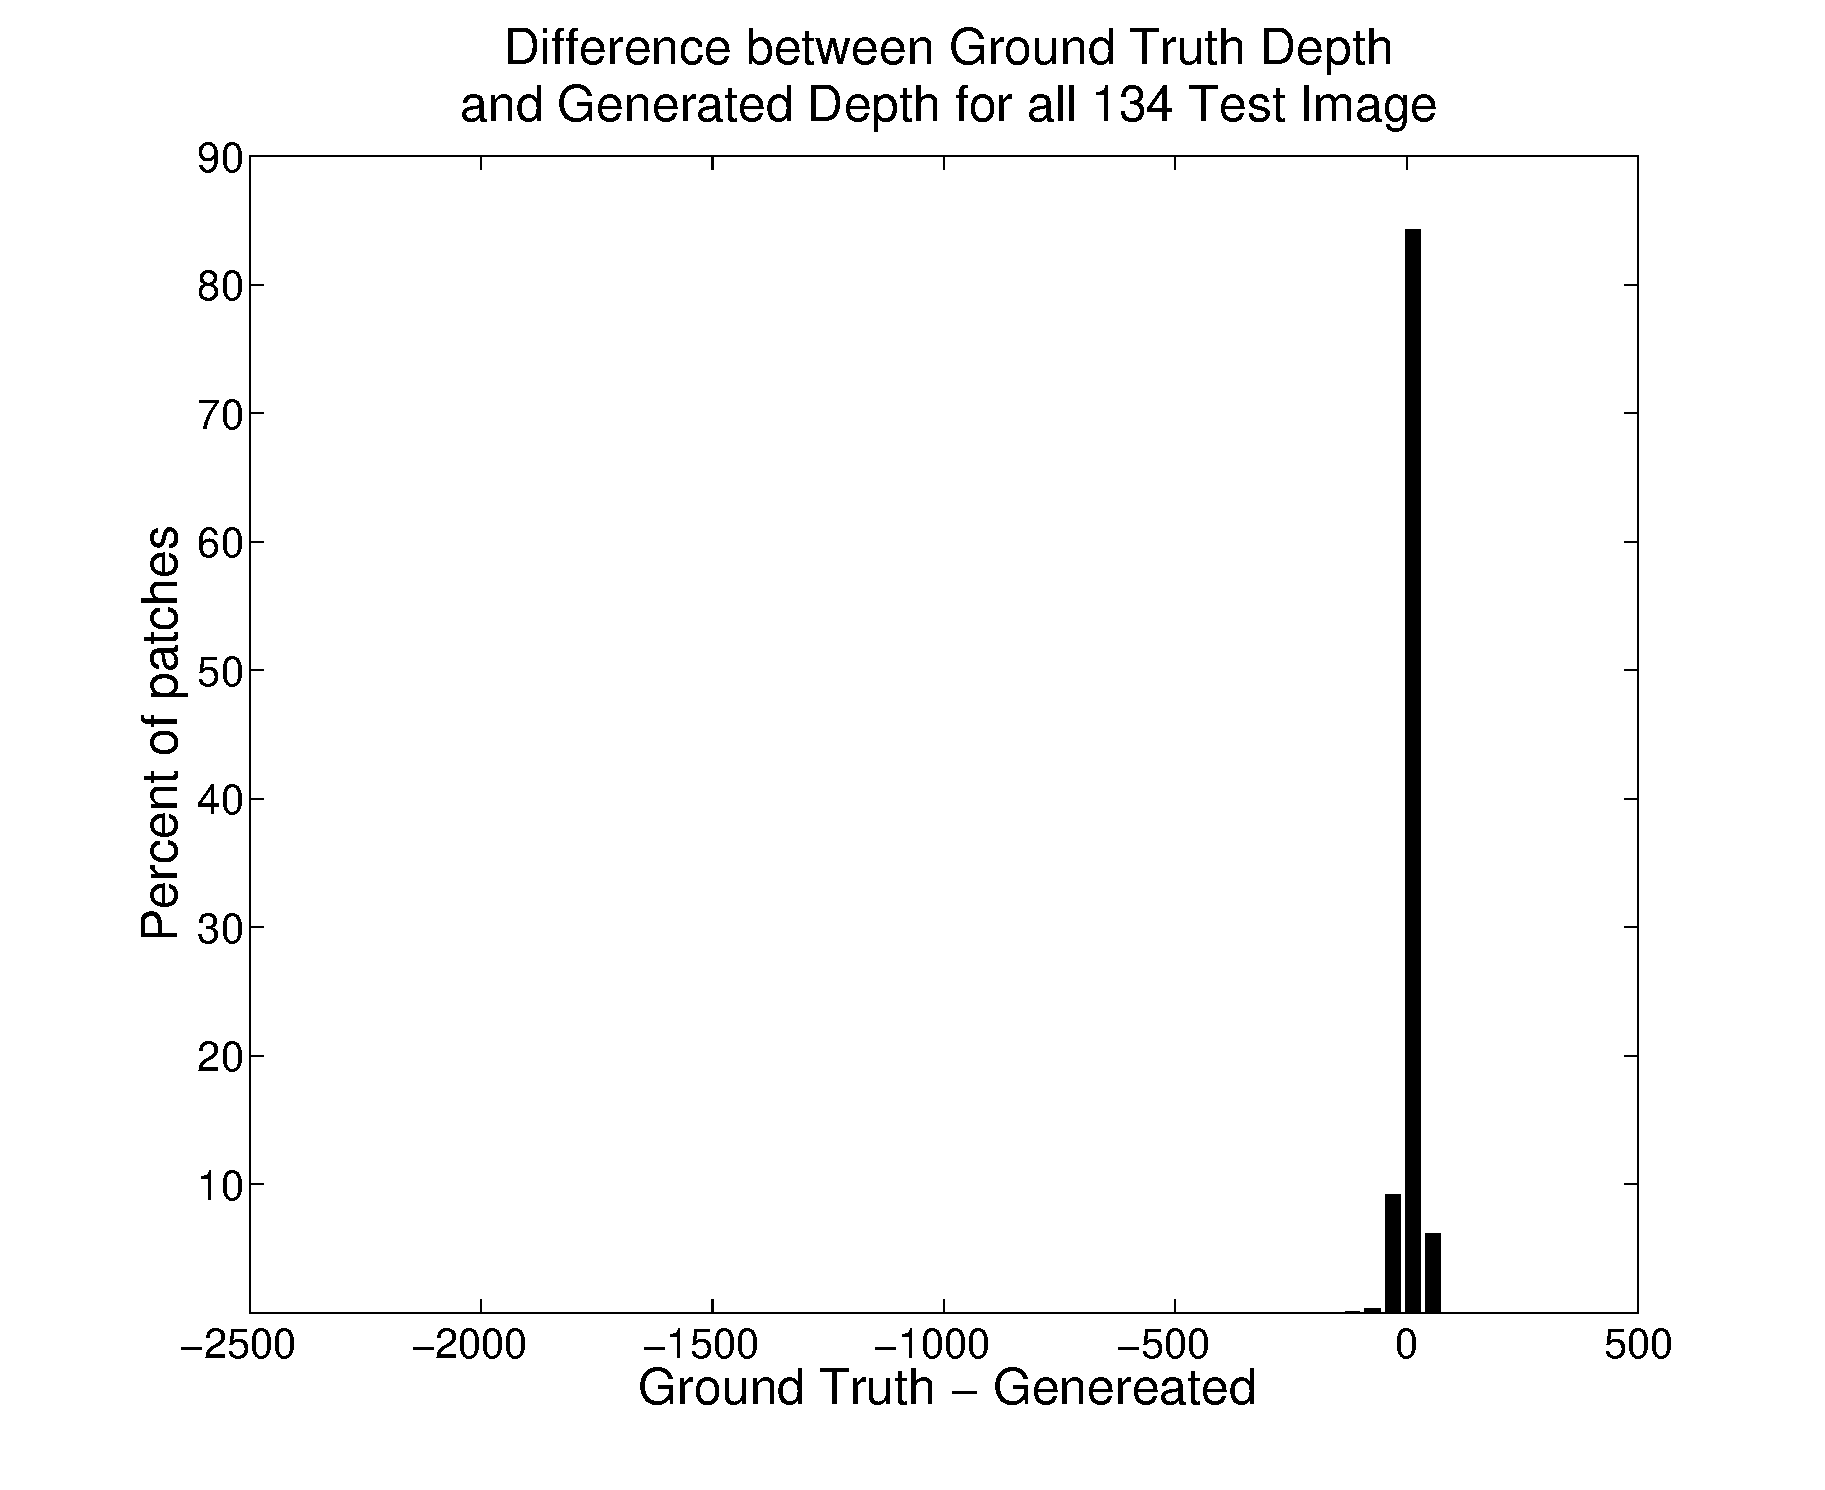
\includegraphics[width=\linewidth]{histogramall10.eps}
\caption{The x axis is the depth error (truth - generated), the y axis is the percent of the patches that fall into this depth error. This is from all the patches of the 134 testing images. This includes all the bins.}
\end{figure}

\begin{figure}
\label{fig:histogramcut}
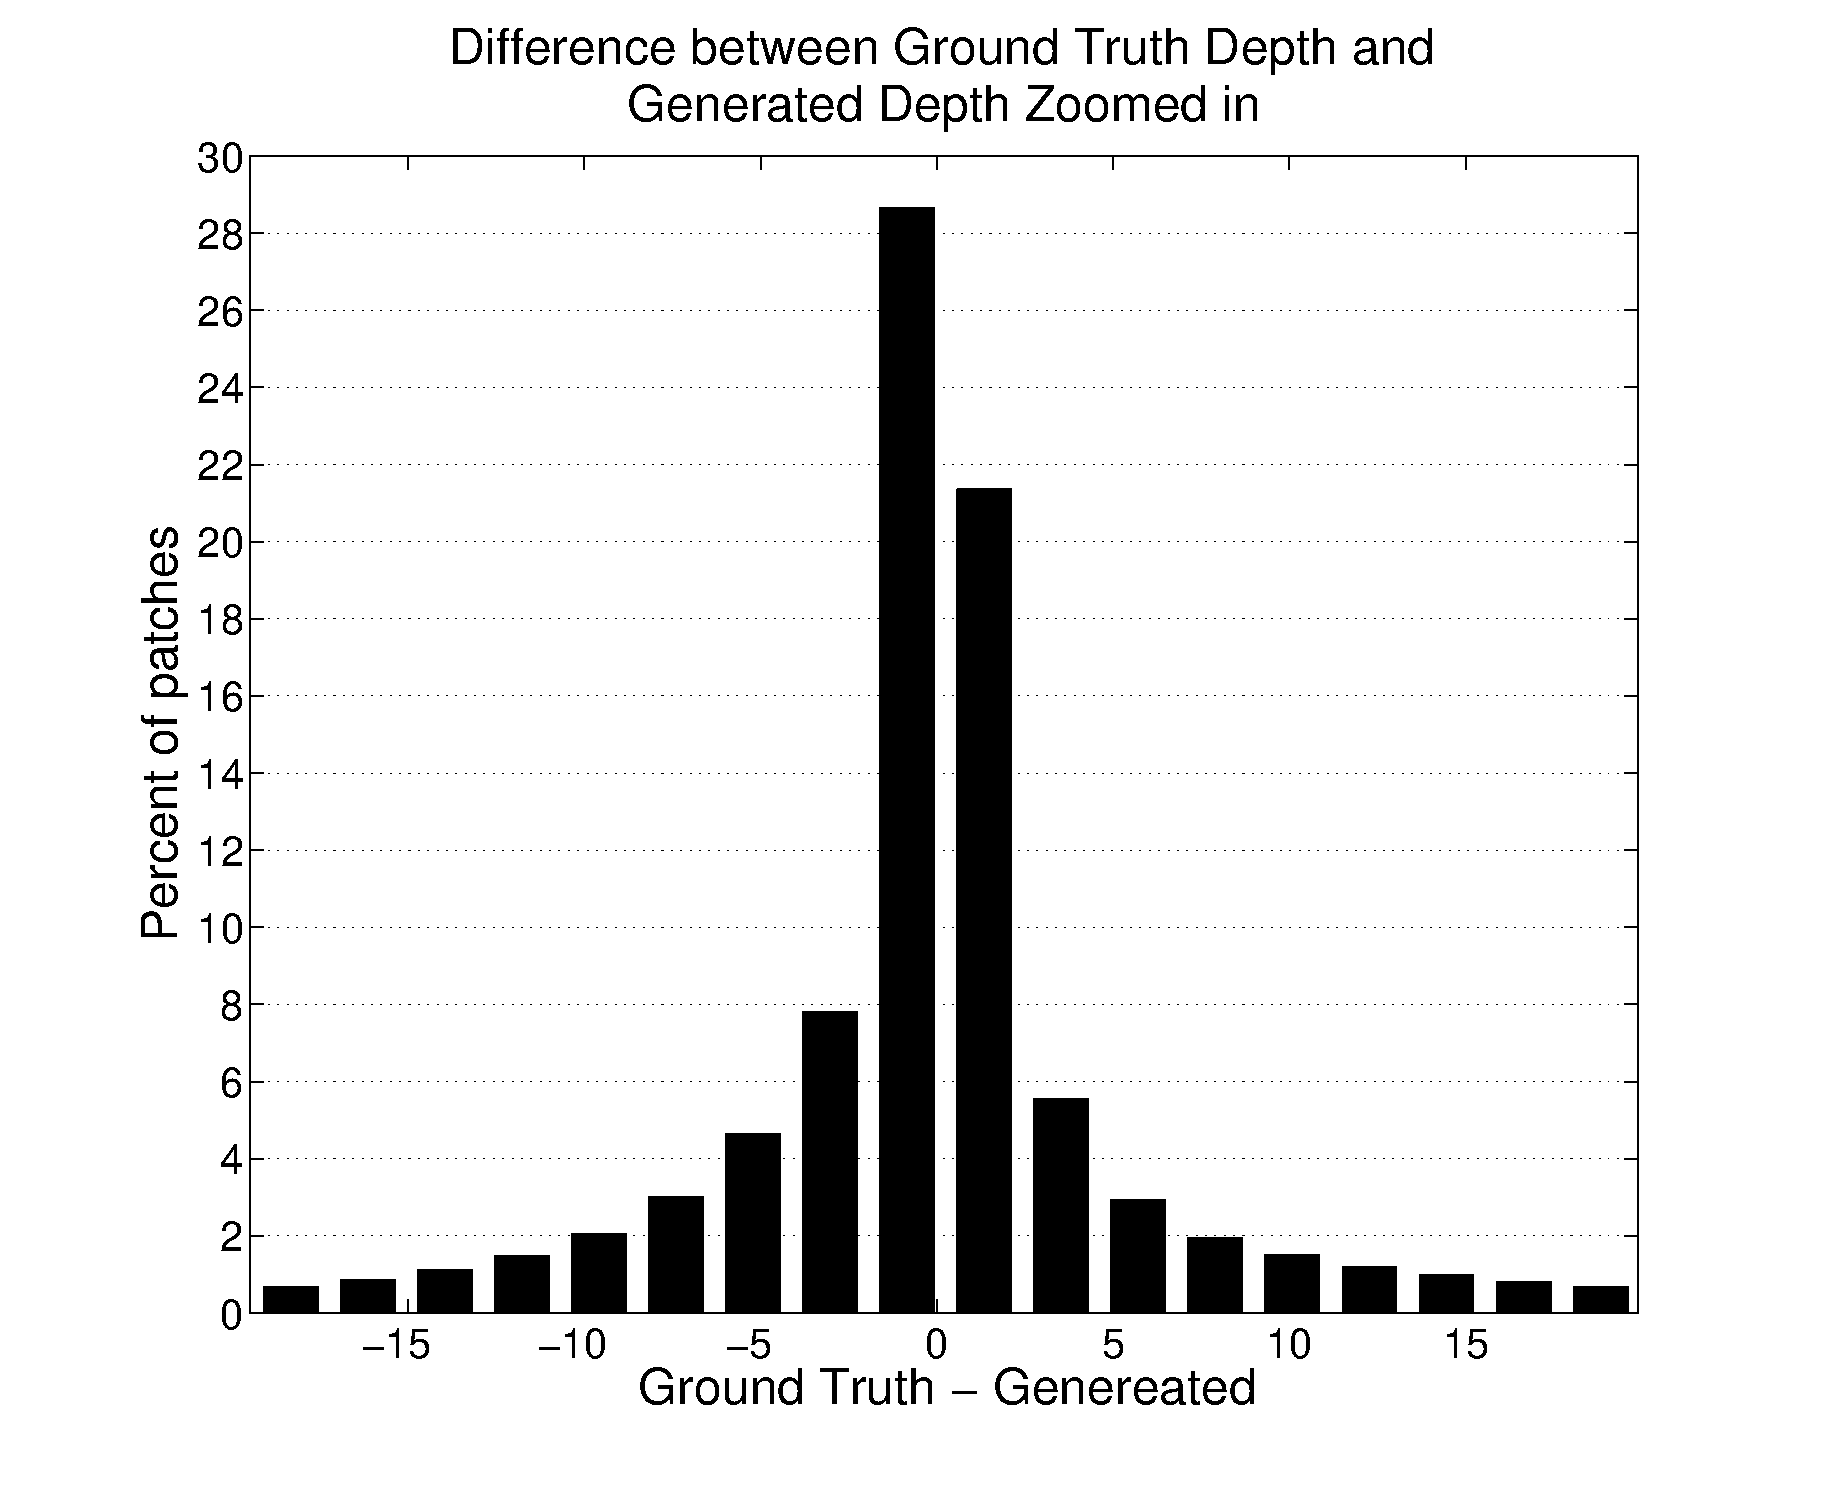
\includegraphics[width=\linewidth]{histogramcut.eps}
\caption{The x axis is the depth error (truth - generated), the y axis is the percent of the patches that fall into this depth error. This is from all the patches of the 134 testing images. This only include the range of bins that from -20 to 20 meters}
\end{figure}

The mean log10 error is very close between the Original and the robust regression of my replication. The difference is to be expected as I'm missing the smoothing terms that come from the relative feature patches, but we can safely say that even without the relative features and smoothing terms that the model still does very well. The least square result is provided to show how much worse it is when we don't remove outliars when we do regression. It actually is still pretty good and provides a 20 times speed up over robust regression. It is interesting to point out that the mean here is only high because there are small numbers of really high differences. If we cut 10\% off the highest difference patches we get a mean error of only 4.072 meters. The histogram of the difference between the real ground truth depth and the generated depth is show in Figure \ref{fig:histogramall10}. This data is generated over 134 testing images, this way we can see what the distribution of the differences. We see that the majority of the error is around 0, but since there are certain errors that are huge, we must zoom in to the relevant areas. Figure \ref{fig:histogramcut} shows the errors that are between -20 and 20 meters. We can see from this that over 80\% of the errors are between -5 and 5 meters and around 60\% of the error is less than -2 to 2 meters. This is pretty good for certain applications such as navigating areas where you can have a huge amount of space you can work in. It is interesting to note that the huge large errors are always negative, this means that the model overestimates the depth more often than it underestimate it. This is due to the linear regression causing certain new data points to force the depth really high. An approach that might fix this is limit the model to the max depth of the laser scanner in training. This removes depths that the training data never could encounter, the point isn't to try and estimate unknown distances using known distances.

\begin{figure*}
\label{fig:comparison}
\centering
\hrule
\vspace{.01in}
{\large Comparison 1} \\
\hrule
\vspace{.1in}
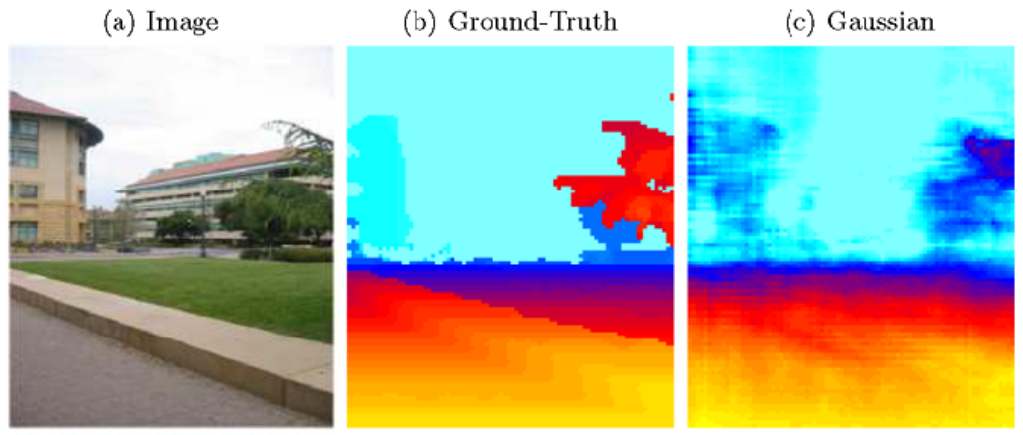
\includegraphics[height=2in]{compare1.png} \\
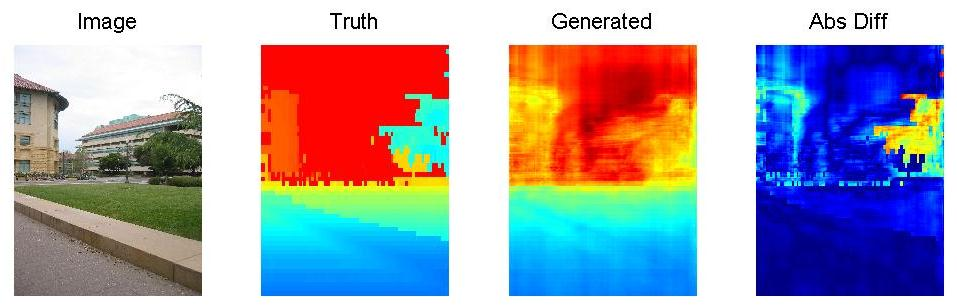
\includegraphics[height=2in]{compare1.jpg} \\
\hrule
\vspace{.01in}
{\large Comparison 2} \\
\hrule
\vspace{.1in}
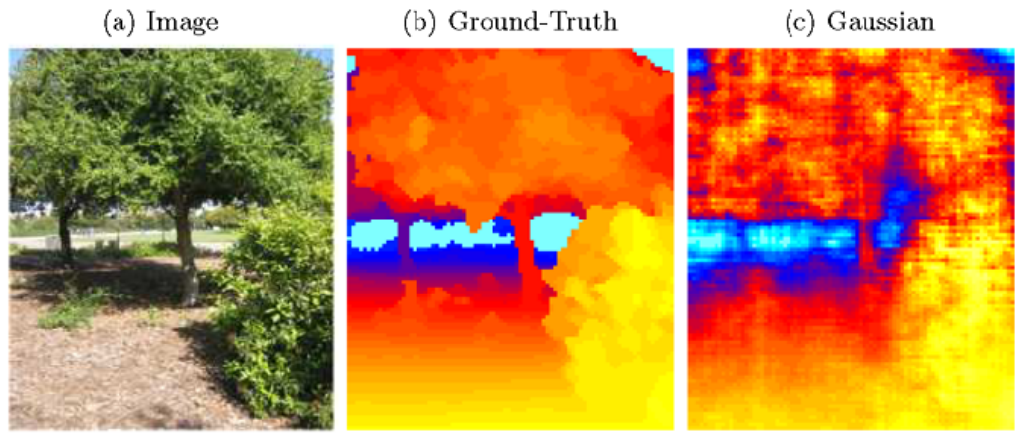
\includegraphics[height=2in]{compare2.png} \\
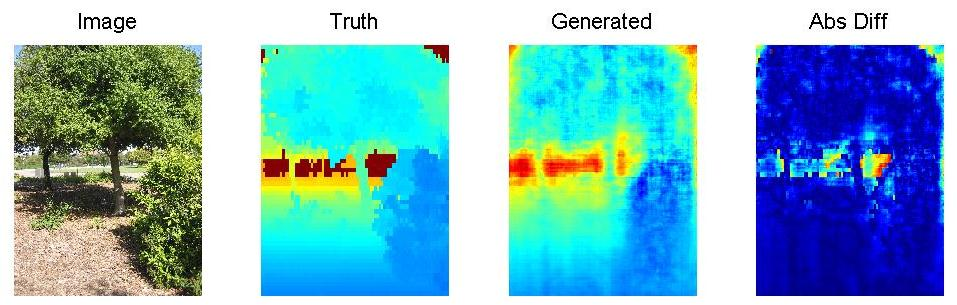
\includegraphics[height=2in]{compare2.jpg} \\
\caption{Comparison between the original result and reproduced result. The top 3 images are the original and the bottom 4 are the reproduction. The colors are inverted from the reproduction and original. The ``Abs Diff'' image is of a different scale than the rest of the images, it's from 0 to the max abs difference in this image.}
\end{figure*}

Even though I used the same testing set as the author, not all of the images they have in their results were in the dataset. Out of the four results that they showed I only found two of them in the dataset I used for training and testing. The comparison results are in Figure \ref{fig:comparison}. All the colors in reversed, this is due to the different scaling that MATLAB uses. 

It is clear that there are certain problems when the smoothing term is removed from the model. If we look in Comparison 1 of Figure \ref{fig:comparison}, at the region that really far away the original results shows the entire area as an uniform far away area, while my result shows that there is a patch in the middle that is even further away than the rest of the sky. This is because in this patch there exists certain cues that cause a further depth, without smoothing information from the surrounding area has a lower effect on the area allowing the weird depth to show up in the results. Notice that both the original and replicated result can't differentiate the tree branches depth from the building depth. I theorize that this is due to the fact that this type of situation doesn't happen in the training set for these feature sets. If we look at Comparison 2 of Figure \ref{fig:comparison}, we see that it does indeed figure out that the bush on the ground is closer. This could just be coincidence as we might have just learned that the closer to the bottom the area is the more likely it is closer. In Comparison 2 we also can note that it does in fact get the stalks of the trees pretty distinctively, and the only huge problem in the difference is the depth of the ``infinite'' area, which usually isn't of high concern.

\begin{figure*}
\label{fig:good}
\centering
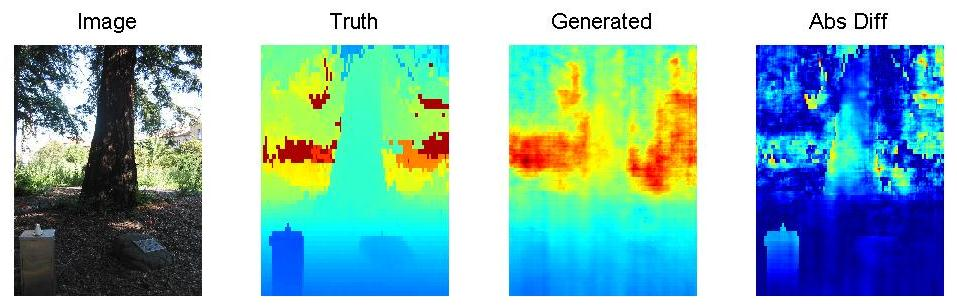
\includegraphics[width=\linewidth]{good1.jpg} \\
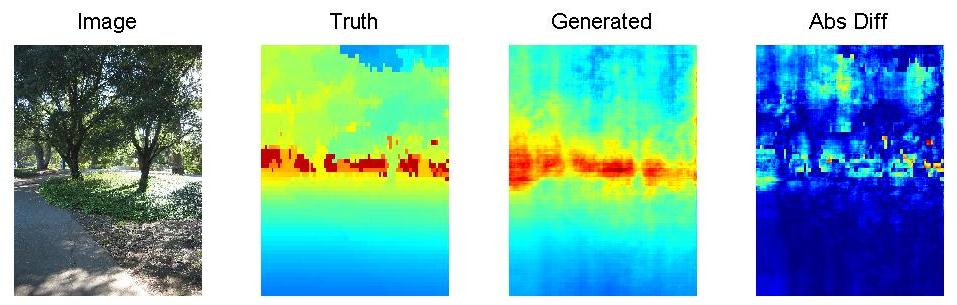
\includegraphics[width=\linewidth]{good2.jpg} \\
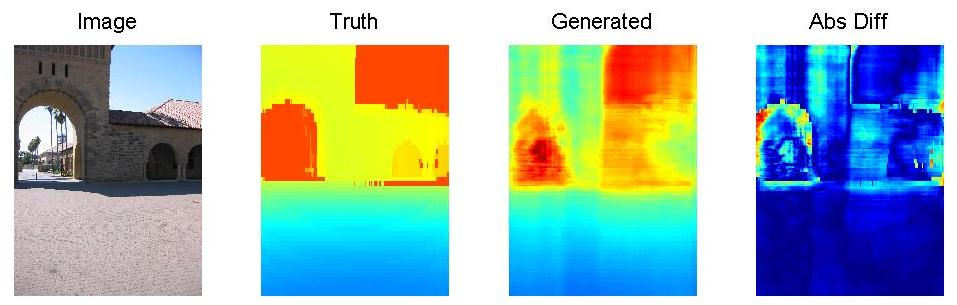
\includegraphics[width=\linewidth]{good3.jpg} \\
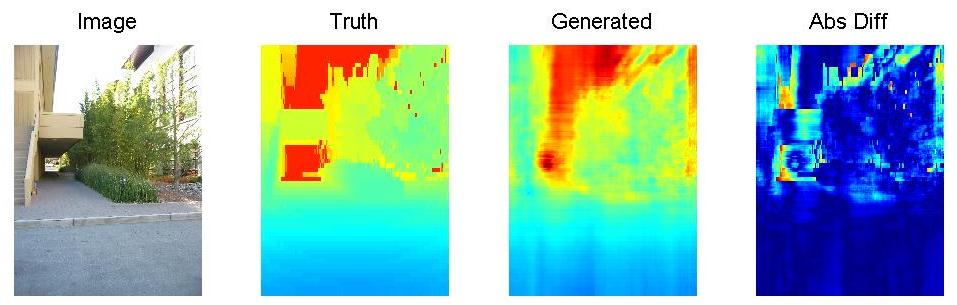
\includegraphics[width=\linewidth]{good4.jpg} \\
\caption{Four extremely good results. The ``Abs Diff'' image is of a different scale than the rest of the images, it's from 0 to the max abs difference in this image.}
\end{figure*}

Figure \ref{fig:good} shows four good results that I extracted from all the results. The first one of the tree is interesting however it gets the stalk from bottom to top. The edge of the tree has the most error, which is expected as this model can't handle instant changes in depth around specific patches. The second image is a good indicator that it can find thin objects such as extremely thing tree stalks, I would argue that this generated depth is almost better than the ground truth from a qualitative point of view. You an clearly see that there are sky bleeding through certain parts of the top of the trees, the laser scanner fails to pick this up as well as this model does. From the four images here we can clearly see the model find the sky pretty consistently, and the ``vanishing poinf'' can be clearly seen with the generated depth map.

\begin{figure*}
\label{fig:bad}
\centering
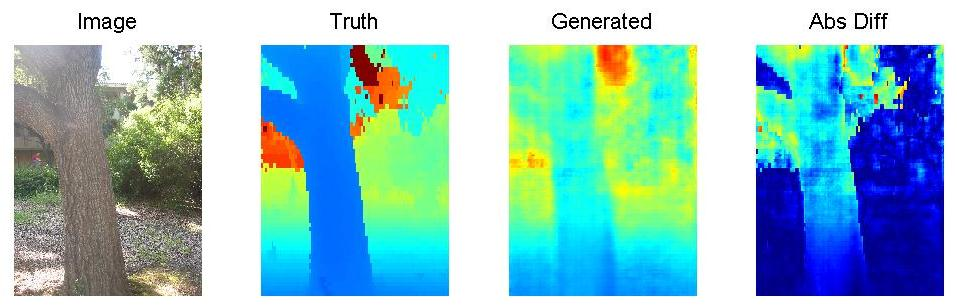
\includegraphics[width=\linewidth]{bad1.jpg} \\
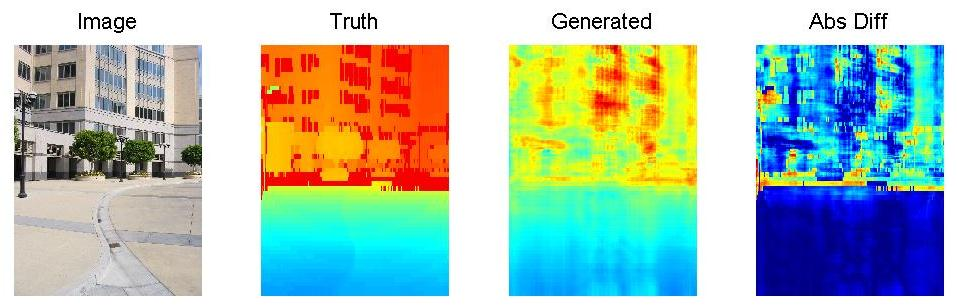
\includegraphics[width=\linewidth]{bad2.jpg} \\
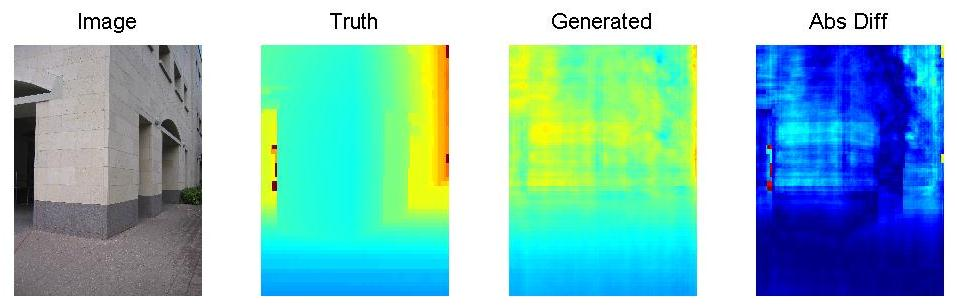
\includegraphics[width=\linewidth]{bad4.jpg} \\
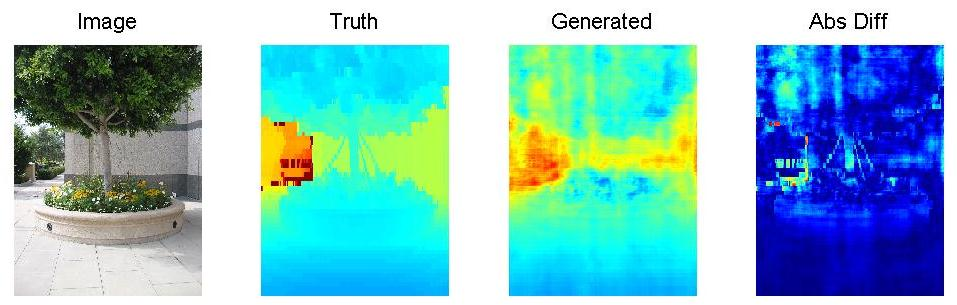
\includegraphics[width=\linewidth]{bad3.jpg} \\
\caption{Four extremely bad results. The ``Abs Diff'' image is of a different scale than the rest of the images, it's from 0 to the max abs difference in this image.}
\end{figure*}

Figure \ref{fig:bad} shows four bad results from the test set. The tree stalk in similar to the one in the Figure \ref{fig:good}, however here it fails to show that the whole stalk is of the same depth, instead it follows the expected result of bottom is closer and top and further away. It completely fails on the two images of the building, and generates a featureless depth map, where the majority of the depth is the same, even though the original images have varying depth in different areas. The last image shows that if there are similar colors or textures for thin objects it will treat as part of the overall larger background, as we lose the stalk of the tree in this image. As I looked at the results I think there are distinct problems that this model cannot handle.

As this is a supervised method, I argue that a image with a swimming pool with the same color as the sky will net the result of the swimming pool being the same distance as the sky. This is because something with similar color to the sky doesn't really exist at all in the training set. If we flip the 3rd image of Figure \ref{fig:good}, we get Figure \ref{fig:flip}. We can tell that this is not a good result at all. This shows that the model is completely reliant on the fact in all of the training images what is closer to the bottom is closer and what is on top is further away. The model can't handle situations that vastly differs from the training set. This might be able to be solved with more training data that cover a wide variety of different situations.

\begin{figure*}
\label{fig:flip}
\centering
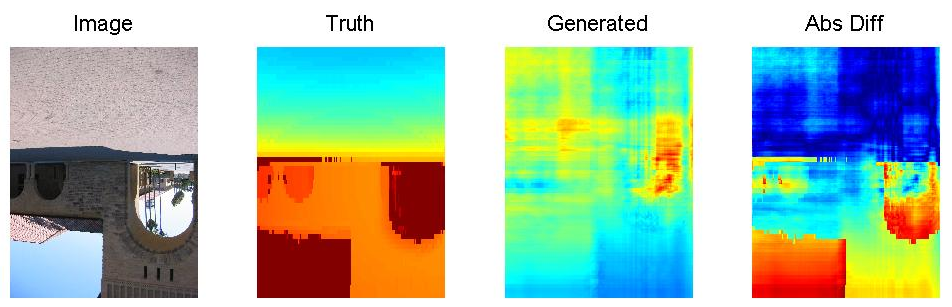
\includegraphics[width=\linewidth]{flip.png}
\caption{}
\end{figure*}

Some other case of the model performing bad is one extremely bright images. As there is no normalization of the intensity the model actually learns specific features that are completely based on the magnitude of the intensity channel. This causes extremely bright objects to be treated as really far away as the sky generally is extremely bright, and that is really far away. This is hard to solve as normalizing unknown scenes is a lot of guessing work. The testing data also shows that extreme close objects are not picked, I'm not sure why this is the case, as the features should be apparent in the training data, however the closer the object is to the camera, it seems more likely that it will generate bogus depth data for at least part of that object. I think a lot of this might have something to do with smoothing but also the information from a local patch doesn't propagate far enough to take advantage of a object that is spanning the whole image. The author does have a newer work that first calculate ``superpixels'' which are just a combination of pixels that are very similar, and then runs a similar MRF model on it \cite{saxenaSU}. This new work does better than the one described in this paper, however it doesn't drastically improve the result.

The speed of this algorithm is not real time, and on-line training can not be added to the model. Training on 400 images takes over 30 hours, and inference takes around 60s. A portion of this can be extremely sped up by using GPUs, since extracting the features from the image is a perfect example of GPU parallel processing. The majority of the training time is the regression algorithm, however that isn't part of the inference, and the inference can also be solved on the GPU. This could potentially speed up the algorithm to real time.

\section{Conclusion}
This method does seem to offer a way to generate depth from a single still image. There are still better ways to generate depth if you are using stereo cameras or a 3d laser scanner. Moving monocular depth generation is better solved by the structure from motion problem. If depth from a single still image is absolutely needed, then this method does give a good estimate to the overall depth map of the image. It can be used to augment the problems plaguing stereo for far away depth, however even then is suffers from a similar problem, features get smaller and more sparse the further away an object is. The method is a good example of just how much information you can extract from a 1MB JPEG image (280MB of information), although how much of that is repetitive is a valid argument.

Some lesson learned is that papers should provide enough information for a person to reproduce the actual result without removing terms that there wasn't enough clarification for. To include a certain term in an equation and give a one sentence unclear description, and not provide a way to calculate this term hinders the reproduction of the paper drastically. While I did get a reproduction working it was not without extreme annoyance at the lack of information about extremely important terms in equations. I also found myself seeking implementation details to actually complete the project in time, certain implementation details might be helpful to include to allow the reproduction to actually be useful. This paper was very hard to reproduce and its merits are few once my reproduction was finished.

\section*{Acknowledgment}
I would like to thank Chansoon Lee, and professor Benjamin Kuipers for helping me with the impossibly hard to understand parameters of the models described in this paper, preventing me from thinking that I was going crazy because nothing made sense.

\bibliographystyle{IEEEtran}
\bibliography{report}

\end{document}